Durch eine Recherche haben sich zwei Arbeiten gezeigt, die sich, analog zu dieser Studienarbeit, mit der künstlichen generierung von Straßenschildern mittels \acp{KNN} beschäftigen. Beide Arbeiten konzentrieren sich darauf, Bildausschnitte zu erzeugen, die ein Straßenschild zeigen und eine geringfügige Menge an Hintergrund um das Schild.

\subsection{Generierung Taiwanischer Straßenschilder mittels DCGAN}
Eine der beiden Arbeiten wurde im Jahr 2021 veröffentlicht. Sie konzentriert sich auf die Generierung taiwanischer Straßenschilder. Dafür wird ein \emph{DCGAN} verwendet, ein \ac{GAN}, das im Generator und im Discriminator eine tiefe \ac{CNN} Architektur besitzt. Getestet wird, inwiefern künstlich generierte Trainingsbilder die Erkennung von Straßenschildern verbessern können. Es werden in der Arbeit vier Arten von Verkehrsschildern generiert. \cite{taiwanGAN}
%\begin{figure}[H]
%   \centering
%   \captionsetup[subfigure]{labelformat=empty}
%   \begin{subfigure}{0.075\textwidth}
%       \centering
%       \includegraphics[height=\textwidth]{../images/Taiwan Schilder/Taiwan_road_sign_禁-25.svg.png}
%       \phantomsubcaption
%   \end{subfigure}
%   \hspace{2em}%
%   \begin{subfigure}{0.075\textwidth}
%       \centering
%       \includegraphics[height=\textwidth]{../images/Taiwan Schilder/600px-Taiwan_road_sign_禁-1.svg.png}
%       \phantomsubcaption
%   \end{subfigure}
%   \hspace{2em}%
%   \begin{subfigure}{0.075\textwidth}
%       \centering
%       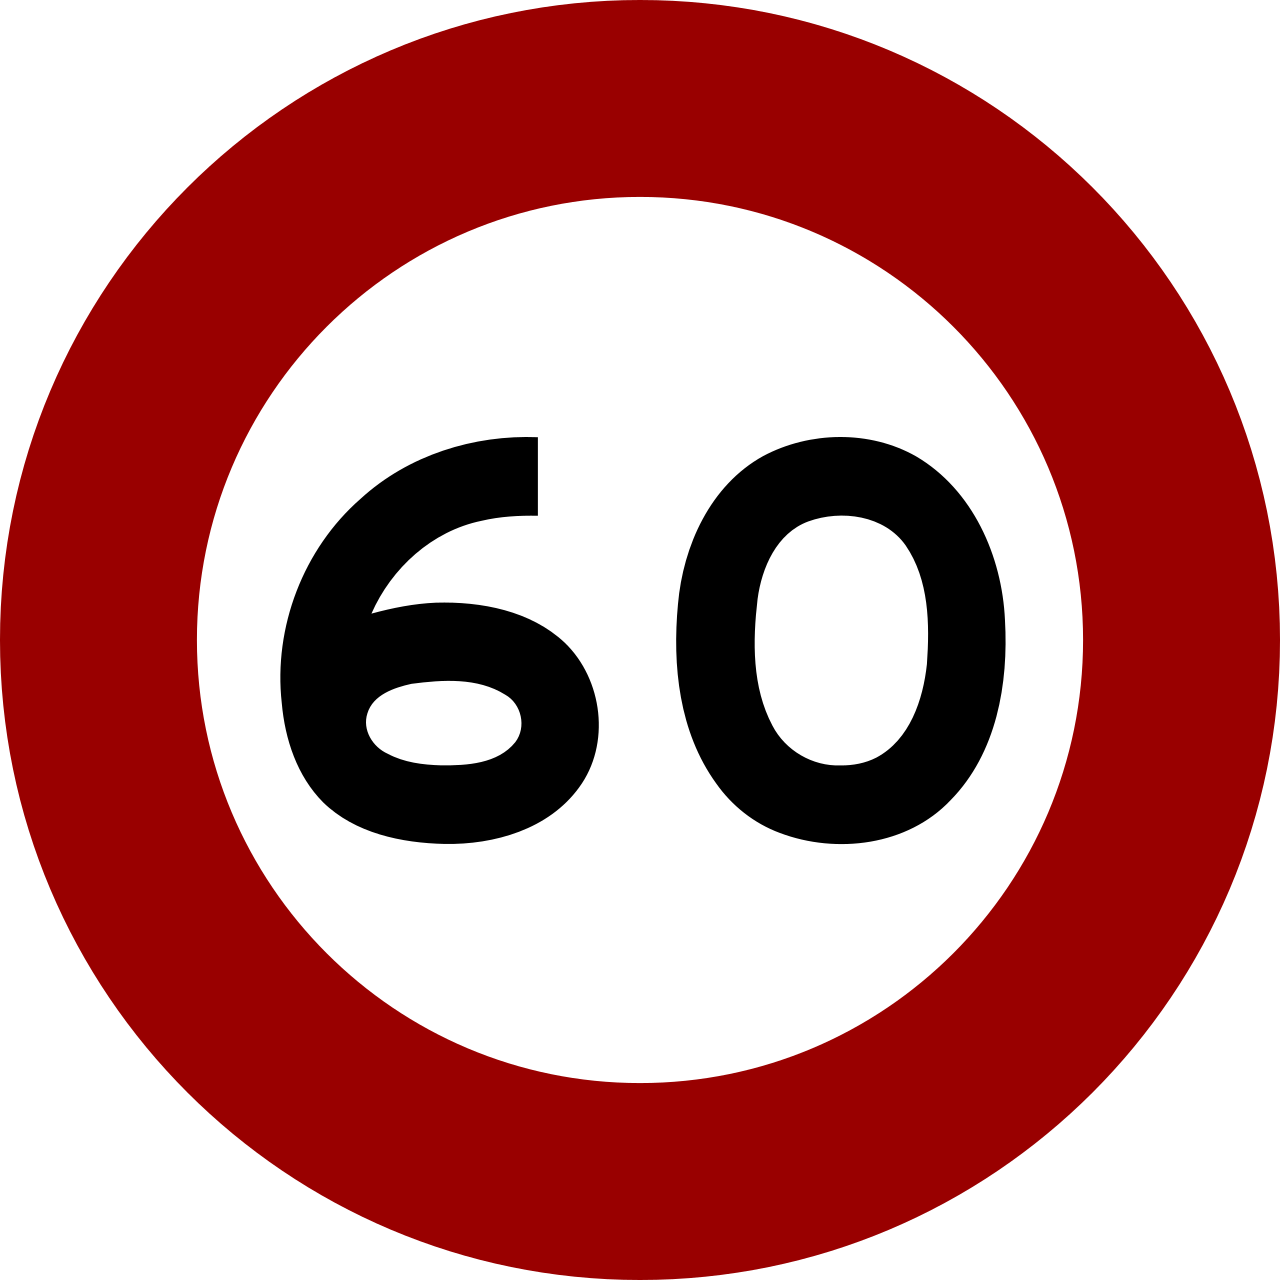
\includegraphics[height=\textwidth]{../images/Taiwan Schilder/Taiwan_road_sign_r5-60.svg.png}
%       \phantomsubcaption
%   \end{subfigure}
%   \hspace{2em}%
%   \begin{subfigure}{0.075\textwidth}
%    \centering
%    \includegraphics[height=\textwidth]{../images/Taiwan Schilder/Taiwan_road_sign_禁-26.svg.png}
%    \phantomsubcaption
%   \end{subfigure}
%      \caption{Generierte Arten von taiwanischen Schildern \cite{taiwanGAN}}
%      \label{fig:taiwan-schilder}
%\end{figure}

Für jede der vier Klassen wird das \ac{GAN} mit 350 Bildern trainiert. Die Bildgrößen variieren dabei, wobei die Maximalgröße bei 200x200 Pixel liegt. Die generierten Bildgrößen korrespondieren zu denen der Trainingsbilder. Es sollen in der Arbeit bewusst keine größeren Bilder als 200x200 Pixel erzeugt werden, da Straßenschilder häufig nur einen kleinen Teil des Sichtfelds auf der Straße ausmachen.
Das Training erstreckt sich auf bis zu 2000 Epochen, was bedeutet, dass das \ac{GAN} während des Trainings 2000 mal alle Trainingsbilder als Eingabe erhält. \cite{taiwanGAN}

Da die Anzahl an Trainingsbildern beschränkt ist, generiert das Modell keine völlig neuartigen Bilder, sondern für jede Klasse jeweils vergleichsweise ähnlich aussehende:

\begin{figure}[H]
    \centering
    \captionsetup[subfigure]{labelformat=empty}
    \begin{subfigure}{0.125\textwidth}
        \centering
        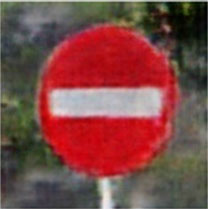
\includegraphics[height=\textwidth]{../images/Taiwan Schilder/Generated0.png}
        \phantomsubcaption
    \end{subfigure}
    \hspace{2em}%
    \begin{subfigure}{0.125\textwidth}
        \centering
        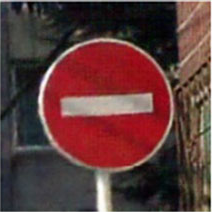
\includegraphics[height=\textwidth]{../images/Taiwan Schilder/Generated1.png}
        \phantomsubcaption
    \end{subfigure}
    \hspace{2em}%
    \begin{subfigure}{0.125\textwidth}
        \centering
        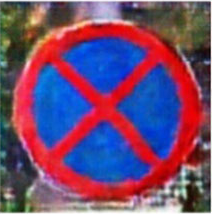
\includegraphics[height=\textwidth]{../images/Taiwan Schilder/Generated2.png}
        \phantomsubcaption
    \end{subfigure}
    \hspace{2em}%
    \begin{subfigure}{0.125\textwidth}
     \centering
     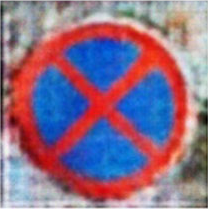
\includegraphics[height=\textwidth]{../images/Taiwan Schilder/Generated3.png}
     \phantomsubcaption
    \end{subfigure}

    %\hspace{2em}%
    \begin{subfigure}{0.125\textwidth}
        \centering
        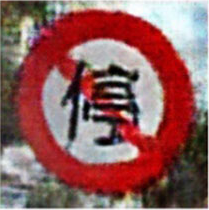
\includegraphics[height=\textwidth]{../images/Taiwan Schilder/Generated4.png}
        \phantomsubcaption
    \end{subfigure}
    \hspace{2em}%
    \begin{subfigure}{0.125\textwidth}
        \centering
        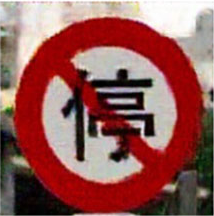
\includegraphics[height=\textwidth]{../images/Taiwan Schilder/Generated5.png}
        \phantomsubcaption
    \end{subfigure}
    \hspace{2em}%
    \begin{subfigure}{0.125\textwidth}
        \centering
        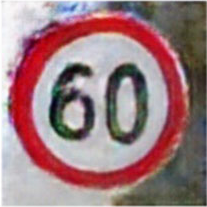
\includegraphics[height=\textwidth]{../images/Taiwan Schilder/Generated6.png}
    \phantomsubcaption
    \end{subfigure}
    \hspace{2em}%
    \begin{subfigure}{0.125\textwidth}
        \centering
        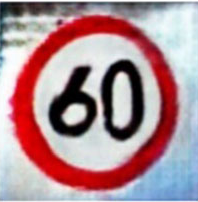
\includegraphics[height=\textwidth]{../images/Taiwan Schilder/Generated7.png}
    \phantomsubcaption
    \end{subfigure}
       \caption{Beispielergebnisse der Generierung taiwanischer SChilder \cite{taiwanGAN}}
       \label{fig:taiwan-gen-schilder}
 \end{figure}

Zur Beurteilung der Generierung wird mitunter der sogenannte \ac{SSIM} verwendet. Statt dass beispielsweise die Differenz aller entsprechenden Pixelwerte berechnet wird, werden hier die Aspekte \emph{Kontrast}, \emph{Leuchtdichte} und \emph{Struktur} der generierten und der echten Bilder verglichen. Dafür werden keine Berechnungen mit einzelnen Pixelwerten durchgeführt, sondern es wird mit den Mittelwerten und der Standardabweichung der Pixelwerte gerechnet. Auf die zugehörigen Formeln wird in Kapitel \ref{chap:Evaluation} eingegangen. \cite{taiwanGAN}

Der Nutzen der generierten Bildern wird anhand eines Modells zur Objektdetektion getestet. In dem Fall, ein sogenanntes \emph{YOLO} Modell. Die Detektion erfolgt auf größeren Bildern, auf denen mehrere Straßenschilder zu sehen sind. Für das Training des Modells werden mit etwa gleicher Gewichtung die für das \ac{GAN} verwendete Trainingsdaten und generierte Daten des \acp{GAN} verwendet. Zur Evaluation wurden hierbei Bilder verwendet, die insgesamt 40 Straßenschilder beinhalten. Die Ergebnisse können folgender Tabelle entnommen werden: \cite{taiwanGAN}

\begin{table}[H]
    \centering
    \begin{tabular}{|l||c|c||l|}
    \hline
    Modell   & \begin{tabular}[c]{@{}c@{}}Reale Trainingsbilder?\end{tabular} & \begin{tabular}[c]{@{}c@{}}Künstliche Trainingsbilder?\end{tabular} & \begin{tabular}[c]{@{}c@{}} Genauigkeit\end{tabular} \\ \hline \hline
    Densenet & Ja                                                                & Ja                                                                    & 92\%                                                                  \\
    Resnet   & Ja                                                                & Ja                                                                    & 91\%                                                                  \\
    Densenet & Ja                                                                & Nein                                                                  & 88\%                                                                  \\
    Resnet   & Ja                                                                & Nein                                                                  & 63\%  \\                                                               
    \hline
    \end{tabular}
    \caption{Vergleich der Objekterkennung mit und ohne künstliche Trainingsdaten}
\end{table}

Das Resultat ist, dass die Erkennung durch die generierten Trainingsdaten verbessert wird. Sowohl das Densenet als auch das Resnet liefern durch sie genauere Ergebnisse. \cite{taiwanGAN}

\subsection{Generierung Deutscher Straßenschilder mittels \acs{CycleGAN}}
\label{chap:vorherige-arbeiten-rub}
Eine weitere Publikation, die sich mit der künstlichen Generierung von Bildern mit Straßenschildern konzentriert, verwendet einen Datensatz, der deutsche Straßenschilder enthält. Er ist unter dem Namen \ac{GTSRB} bekannt. Auf den Datensatz wird näher in Kapitel \ref{chap:konzept} eingeganen, da er auch die Basis für diese Arbeit bildet. Die genannte Publikation ist aus einer Masterarbeit an der Ruhr Universität Bochum entstanden. Dort wurde auch der \ac{GTSRB} veröffentlicht. 

Die Architektur des Modells ist hier eine andere als bei der bisher beschriebenen Generierung taiwanischer Schilder. In dieser Arbeit wird ein \ac{CycleGAN} statt eines \emph{Vanilla \acp{GAN}} verwendet. Die beiden Generatoren basieren auf einem Resnet. \cite{GTSRB} \cite{gtsrbGAN}

Für die Generierung erhält das Netzwerk das Piktogramm eines Straßenschilds als Eingang. Das \ac{CycleGAN} soll einen möglichst realistisch wirkenden Hintergrund um das Straßenschild erzeugen. Vor der Generierung werden die Piktogramme der Straßenschilder zufällig rotiert und ein zufälliger einfarbiger Hintergrund erzeugt. Letzteres soll eine weitere stochastische Komponente für die Generierung bilden, damit eine größere Varianz an Hintergründen erzeugt wird. Für das Training des Netzes verwendet die Arbeit eine präparierte Version des \ac{GTSRB}. Der Datensatz beinhaltet dadurch folgende Eigenschaften:
\begin{itemize}
    \item Nur Bilder mit einer Mindestauflösung von 64x64 Pixeln werden verwendet
    \item Die Bilder werden so zugeschnitten, dass sie quadratisch sind
    \item Die Klassen werden ausbalanciert, um der asymmetrischen Verteilung an Trainingsbildern pro Klasse entgegenzuwirken
    \item Insgesamt besteht der präparierte Datensatz aus 12.212 Bildern
  \end{itemize}
\cite{gtsrbGAN}

\textbf{generierte Beispiele einfügen}

Es erfolgt eine Evaluation, inwiefern die künstlich generierten Trainingsbilder zwei verschiedene Klassifikatoren verbessern können. Dabei handelt es sich um eine sogenannte \ac{SVM} und ein \ac{CNN}. \acp{SVM} sind eine Art von trainierbaren Klassifikatoren, die nicht auf \acp{KNN} basieren \cite{visualApproach}. Einerseits werden die Algorithmen mit realen Trainingsdaten trainiert und andererseits vollständig mit generierten Daten. Die Ergebnisse bezüglich der Genauigkeit der Klassifikation je nach der Art der Trainingsbilder ist in Tabelle \ref{tab:cyclegan-eval} dargestellt. Es lässt sich erkennen, dass die Klassifikation um jeweils etwa 7-9\% ungenauer ist, als mit realen Trainingsdaten. Es ist jedoch auch erwartbar, dass die Genauigkeit etwas geringer ausfällt, da die generierten Bilder der Verteilung des echten Trainingsdatensatzes folgen sollen, dies jedoch nicht zu 100\% möglich ist. \cite{gtsrbGAN}

\begin{table}[H]
    \centering
    \begin{tabular}{|l||c|c||l|}
    \hline
    Modell & \begin{tabular}[c]{@{}c@{}}Reale Trainingsbilder?\end{tabular} & \begin{tabular}[c]{@{}c@{}}Künstliche Trainingsbilder?\end{tabular} & \begin{tabular}[c]{@{}c@{}}Genauigkeit\end{tabular} \\ \hline \hline
    CNN    & Ja                                                                & Nein                                                                  & 95,42\%                                                               \\
    SVM    & Ja                                                                & Nein                                                                  & 87,97\%                                                               \\
    CNN    & Nein                                                              & Ja                                                                    & 87,57\%                                                               \\
    SVM    & Nein                                                              & Ja                                                                    & 79,27\% \\
    \hline                                                              
    \end{tabular}
    \caption{Vergleich der Klassifikation mit echten und künstlichen Trainingsdaten \cite{gtsrbGAN}}
    \label{tab:cyclegan-eval}
\end{table}